\chapter{Projekt Organisation}
\begin{figure}[ht]
    \center
    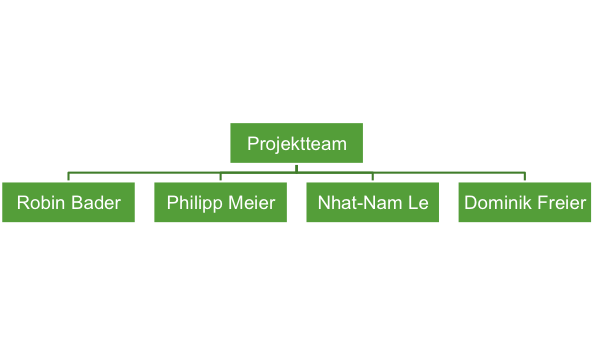
\includegraphics[width=0.8\textwidth]{content/images/projekt_organisation.png}
    \caption{Projekt Organisation}
\end{figure}

\section{Organisationsstruktur}
Nachfolgend die involvierten Personen und ihre Funktionen.
    \begin{table}[H]
        \tablestyle
        \tablealtcolored
        \begin{tabularx}{\textwidth}{l X X l}
        \tableheadcolor
            \tablehead Name & 
            \tablehead Funktion(en) & 
            \tablehead Kontakt & 
            \tablehead Bemerkungen \\  
        \tablebody
            Dominik Freier & Software-Entwickler & \href{mailto:dfreier@hsr.ch}{dfreier@hsr.ch} \linebreak +41 78 647 87 87 & \tabularnewline 
            Nhat-Nam Le & Software-Entwickler \linebreak Serveradministrator & \href{mailto:nle@hsr.ch}{nle@hsr.ch}  \linebreak +41 79 563 34 09 & \tabularnewline 
            Philipp Meier & Software-Entwickler & \href{mailto:p1meier@hsr.ch}{p1meier@hsr.ch} \linebreak +41 79 654 61 09 & \tabularnewline 
            Robin Bader & Software-Entwickler & \href{mailto:r1bader@hsr.ch}{r1bader@hsr.ch} \linebreak +41 79 294 24 78 & \tabularnewline 
        \tableend
        \end{tabularx} 
    	\caption{Organisationsstruktur}
    \end{table}
    
\section{Verantwortlichkeiten}
Dem Projekt stehen vier gleichgestellte Entwickler gegenüber. Um Abhängigkeiten zu Personen zu vermeiden, soll das Know-how über alle Entwickler verteilt werden.
Zuständigkeiten werden daher nicht explizit ausgesprochen und nur Tasks während den Iterationen zugewiesen.
Einzig die Ansprechsperson wird definiert.
    \begin{table}[H]
        \tablestyle
        \tablealtcolored
        \begin{tabularx}{\textwidth}{l X}
        \tableheadcolor
            \tablehead Wer & 
            \tablehead Verantwortlichkeiten \tabularnewline  
        \tablebody
            Dominik Freier & Planung, Infrastruktur, Entwicklung \tabularnewline 
            Nhat-Nam Le & Planung, Infrastruktur, Entwicklung \tabularnewline 
            Philipp Meier & Planung, Infrastruktur, Entwicklung, \textbf{Ansprechsperson} \tabularnewline 
            Robin Bader & Planung, Infrastruktur, Entwicklung \tabularnewline 
        \tableend
        \end{tabularx} 
    	\caption{Verantwortlichkeiten}
    \end{table}

\section{Externe Schnittstellen}
\textbf{Betreuer:} Luc Bläser
\\
\textbf{Weitere Betreuer:} Hans Rudin und Daniel Keller

Herr Bläser wird das Projekt betreuen und Reviews durchführen. Für Fragen oder andere Anliegen können auch die übrigen Anspruchspersonen beigezogen werden.
